\chapter{Introducción Específica} % Main chapter title

\label{Chapter2}

Es este capítulo se presentan las topologías típicas del sistema ferroviario y los enfoques de resolución, con sus ventajas y desventajas antes de abordar la implementación de la solución elegida.

\section{Topologías típicas}
\label{Topologias}	
	El tendido ferroviario argentino dista de ser uniforme: en las zonas rurales predominan vías simples con bypass debido al alto costo de utilizar vías dobles, mientras que en las zonas urbanas son mayoría las estaciones y playas de maniobras a talleres de mantenimiento.
	
	Es por eso que el trabajo realizado debe abocarse a muchas locaciones y muy diversos unos de otros. La cantidad de elementos involucrados incrementa conforme la complejidad de la topología aumenta, pero los elementos y sus comportamientos no dejan de ser los mismos de los presentados en el capítulo 1.

	\subsection{Bypass}

		Para cubrir grandes distancias entre un punto estratégico, como podría ser Vaca Muerta, y un puerto para la exportación de los recursos se requiere una línea ferroviaria con vagones de carga que puedan transportar el producto. Por supuesto, es necesario un ida y vuelta entre trenes vacíos que van a ser llenados en el destino y trenes llenos que van a descargar al puerto la carga que lleven, pero el costo de utilizar dos vías en sentidos opuestos es muy elevado y usar solo una no tiene el menor sentido logístico.
		
		Es por eso que se utiliza la topología de bypass cada cierta cantidad de kilómetros de vías simples para poder permitir que trenes en sentidos opuestos se crucen sin riesgo de colisión. En la figura \ref{fig:Bypass_2} se representa la topología bypass, donde un tren que circula hacia la derecha por la vía principal podría entrar en colisión lateral con un tren que busca ingresar a la red desde una vía secundaria por medio del cambio de vías.
		
		\begin{figure}[h]
		\centering
			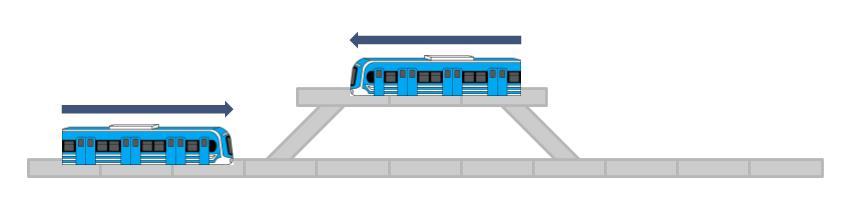
\includegraphics[scale=.45]{./Figures/Bypass_2}
			\caption{Topología bypass.}
			\label{fig:Bypass_2}
		\end{figure}

	\vspace{5cm}
				
	\subsection{Estación}

		Los lugares donde se habilita a los pasajeros a ingresar o salir del tren se denominan andenes y se encuentran en las estaciones ferroviarias situadas cada cierta cantidad de kilómetros, en diferentes localidades del país. En la figura \ref{fig:Estacion} se muestra una topología de estación simple con andén central. Es decir, el mismo andén permite utilizar trenes tanto de la vía ascendente como de la descendente. Se añadió un paso a nivel vehicular en las inmediaciones de la estación y dos cambios de vías en orientaciones opuestas para permitir a la formación realizar trayectos cortos entre terminales, utilizando la estación como terminal provisoria.
		
			\begin{figure}[h]
			\centering
				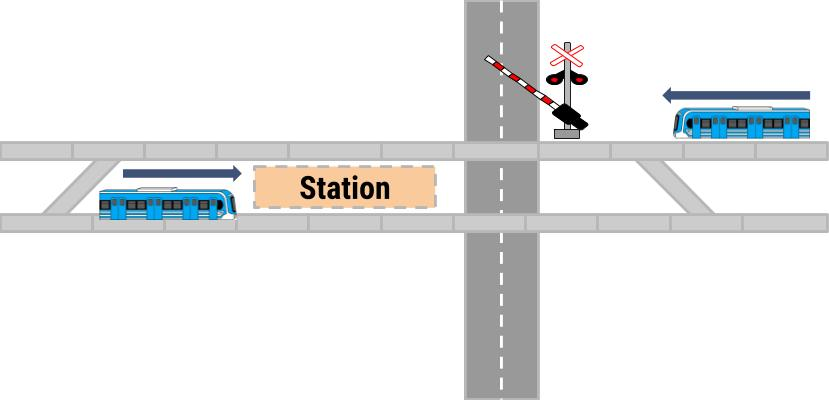
\includegraphics[scale=.45]{./Figures/Estacion}
				\caption{Topología estación con andén único.}
				\label{fig:Estacion}
			\end{figure}
		
		Aunque estaciones de andén único como la estación de Gerli de la Línea Roca son comunes, también existen estaciones con dos andenes: uno puramente para utilizar la vía ascendente y alejarse de la terminal, y otro puramente descendente para viajar hacia la terminal. Tal es el caso de estaciones como Longchamps, Adrogué, Remedios de escalada de la Línea Roca.

	\subsection{Hub}
	
		Otras topologías mas complejas incluyen una cantidad extra de andenes, como Lomas de Zamora o Temperley, que pueden recibir formaciones de varios ramales distintos (Glew/A. Korn, Ezeiza, Bosques, Quilmes, La Plata, etc.) o incluso tener accesos a playas de maniobras o talleres de reparación para poder inyectar o retirar formaciones de la red. Tal es el caso representado en la figura \ref{fig:Hub}, donde se tiene una mayor cantidad de andenes, ingresos/egresos a talleres ferroviarios o bifurcaciones a otros ramales, además de la rama principal de circulación entre terminales. 
		
			\begin{figure}[h]
			\centering
				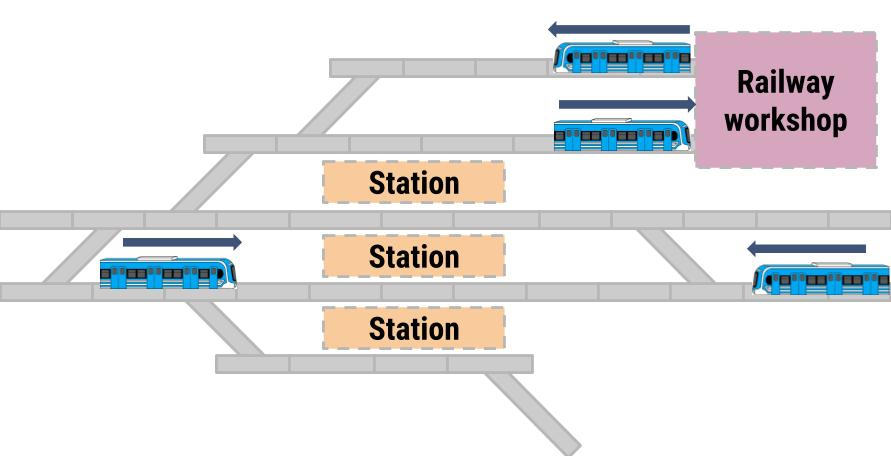
\includegraphics[scale=.44]{./Figures/Hub}
				\caption{Topología hub.}
				\label{fig:Hub}
			\end{figure}
	
		Un buen ejemplo de esta topología es la estación Llavallol de la Línea Roca. En ella se tiene una extensa playa de maniobras como la comandada por el panel de control de la figura \ref{fig:Electromecanico}.
		
	\subsection{Terminal}
		
		Finalmente, la topología mas compleja de todas es la denominada terminal, tal como se representa en la figura \ref{fig:Terminal}. En ella se encuentran numerosos andenes que pueden ser tanto de ingreso como de egreso indistintamente, presentan muchos cambios de vías para facilitar el intercambio de formaciones y permitir que las vías funcionen en ambos sentidos de circulación, además de tener ramificaciones para diversos ramales que convergen en la terminal.
		
			\begin{figure}[h]
			\centering
				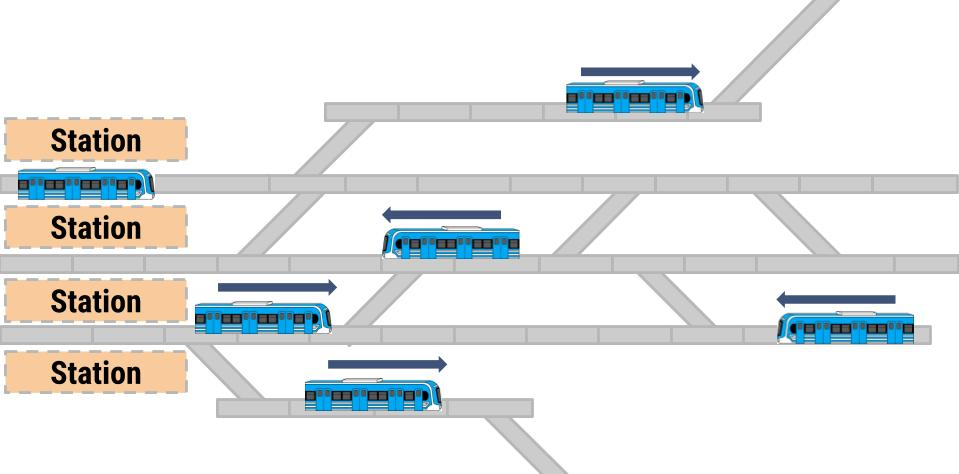
\includegraphics[scale=.4]{./Figures/Terminal}
				\caption{Topología terminal.}
				\label{fig:Terminal}
			\end{figure}
		
		Ejemplos de esta topología pueden ser las estaciones Once de septiembre (Línea Sarmiento), Alejandro Korn y Constitución (Línea Roca) o Retiro (Línea San Martín, Línea Mitre, Línea Belgrano Norte y Cargas). Incluso hay estaciones que, aunque no son el final del recorrido, pueden funcionar como terminales de ramales mas cortos tales como Ezeiza, que extiende el ramal Constitución-Ezeiza hasta Cañuelas, o Glew, que extiende el ramal Constitución-Glew hasta Alejandro Korn.
		

\section{Estrategias de resolución}
	\label{2_2}
	A lo largo de la investigación se relevaron decenas de artículos, los cuales abordan el problema con dos estrategias de desarrollo muy diferenciadas, cada una con sus ventajas y desventajas: el enfoque funcional y el enfoque geográfico.
	
	En el enfoque funcional, el desarrollo se basa en la denominada "tabla de enclavamientos". La tabla de enclavamientos define las condiciones que deben cumplirse para habilitar cada una de las rutas posibles. Cada itinerario se forma a partir de la conjunción de diferentes rutas, siempre que estas sean compatibles, lo cual también está indicado en la tabla. Este concepto se ampliará en la sección \ref{Tabla_Enclavamientos}.
	
	Históricamente, tanto los enclavamientos mecánicos como los electromecánicos se han definido previamente por tablas de enclavamientos, las cuales también pueden ser usadas para definir la logística de la red. Es por eso que el personal técnico está muy capacitado tanto en la lectura de la tabla como en su elaboración. 
	
	En el enfoque geográfico, en cambio, no hay una descripción macro del sistema a nivel funcional, sino una descripción a nivel de componentes. Es la interacción entre los componentes, en función de su posición geográfica en el entorno, lo que se manifiesta a nivel macro. De poder definir las reglas genéricas de cada elemento y las condiciones en las cuales interactúan, es posible definir cualquier sistema, sin tabla de enclavamientos.
	
	Este enfoque dista de ser inmediato, ya que es necesario construir todas las herramientas de análisis de la red y diseñar cada elemento al detalle. La ventaja es que, concluida esa etapa, se independiza el enfoque de la locación, logrando una solución más flexible. Además de definir todas las funcionalidades que la red admite y no solo las necesarias para la logística.
	
	En las siguientes secciones se profundizará en ambos enfoques, los conceptos necesarios para su plena comprensión, cómo se modifica el flujo de trabajo y el análisis de su escalabilidad. Esto último es de vital importancia a la hora de comparar ambos enfoques.
	
	
% Describirlas
% flujo de trabajo, modelo , escalabilidad explicado ANTES
% enfoque funcional > historico, muy utilizado

\section{Enfoque funcional}
	\label{Incompletitud}

	El concepto de tabla de enclavamientos\cite{cite21,cite22} se introdujo en forma resumida en la sección \ref{2_2}. Sin embargo, dado que es fundamental para entender el enfoque funcional, a continuación se lo describe en detalle.%, para luego seguir explicando los demás elementos del enfoque funcional a partir de la sección \ref{2_3_2}.
		
	\subsection{Tabla de enclavamientos}
	\label{Tabla_Enclavamientos}
		A la hora de establecer itinerarios se utiliza el concepto de ruta, que es el camino definido entre dos semáforos consecutivos. Pero no siempre se establecen todas las rutas posibles, sino solo las necesarias para generar los itinerarios. Por ejemplo, en la figura \ref{fig:EJ_Tabla} se pueden ver dos casos de definición de rutas para una misma topología de bypass.
		
			\begin{figure}[h]
			\centering
				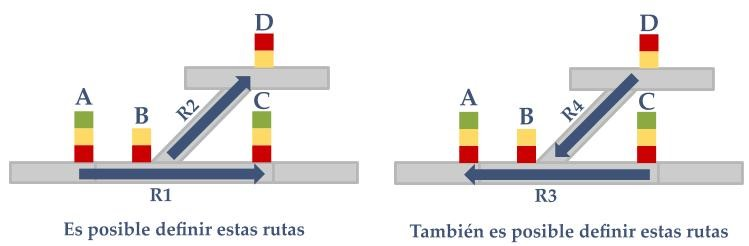
\includegraphics[scale=.65]{./Figures/Tablas}
				\caption{Ejemplo de elaboración de las rutas.} 
				\label{fig:EJ_Tabla}
			\end{figure}
		
		En el primer caso se indican las rutas que corresponden a utilizar las vías en el sentido de izquierda a derecha. Para la ruta $\text{R}_1$ el semáforo A es el inicial y el semáforo C es el final. Para la ruta $\text{R}_2$ el semáforo de maniobra B es el inicial y el semáforo de maniobra D es el final. Esto se presenta en la Tabla \ref{Tabla_simple}.
		
		\begin{table}[!hbt]
		\renewcommand{\arraystretch}{1.3}
	
		\caption{Tabla de enclavamientos (izquierda a derecha)}
		\label{Tabla_simple}
		\centering
	
		\begin{tabular}{c c c c c c c}
		\hline
		Ruta & Señal de entrada & Señal de salida \\
		\hline
		 1 & $\text{Semáforo}_A$  & $\text{Semáforo}_C$ \\
		 2 & $\text{Semáforo}_B$  & $\text{Semáforo}_D$ \\
		\hline
		\end{tabular}
		\end{table}
		
		En el segundo caso de la figura \ref{fig:EJ_Tabla} el itinerario podría contemplar también un uso estrictamente de derecha a izquierda. Sumando así las rutas $\text{R}_3$ y $\text{R}_4$, como se describe en la Tabla \ref{Tabla_bidireccional}.
		
		\begin{table}[!hbt]
		\renewcommand{\arraystretch}{1.3}
	
		\caption{Tabla de enclavamientos (derecha a izquierda)}
		\label{Tabla_bidireccional}
		\centering
	
		\begin{tabular}{c c c c c c c}
		\hline
		Ruta & Señal de entrada & Señal de salida \\
		\hline
		 3 & $\text{Semáforo}_C$  & $\text{Semáforo}_A$ \\
		 4 & $\text{Semáforo}_D$  & $\text{Semáforo}_B$ \\
		\hline
		\end{tabular}
		\end{table}
		
		Según el uso que se le quiera dar a la topología, ambas tablas de enclavamientos son válidas. Incluso podemos notar que ambas están incompletas porque una tabla no contempla los casos de la otra. Se puede definir entonces una nueva tabla de enclavamientos como la conjunción de ambas, como se describe en la Tabla \ref{Tabla_total}.
		
		\begin{table}[!hbt]
		\renewcommand{\arraystretch}{1.3}
	
		\caption{Tabla de enclavamientos (caso bidireccional)}
		\label{Tabla_total}
		\centering
	
		\begin{tabular}{c c c c c c c c }
		\hline
		Ruta & Señal de entrada & Señal de salida & Rutas conflictivas \\
		\hline
		 1 & $\text{Semáforo}_A$  & $\text{Semáforo}_C$ & $\text{R}_2$, $\text{R}_3$ y $\text{R}_4$ \\
		 2 & $\text{Semáforo}_B$  & $\text{Semáforo}_D$ & $\text{R}_1$, $\text{R}_3$ y $\text{R}_4$ \\
		 3 & $\text{Semáforo}_C$  & $\text{Semáforo}_A$ & $\text{R}_1$, $\text{R}_2$ y $\text{R}_4$ \\
		 4 & $\text{Semáforo}_D$  & $\text{Semáforo}_B$ & $\text{R}_1$, $\text{R}_2$ y $\text{R}_3$ \\
		\hline
		\end{tabular}
		\end{table}
		
		Se añade a la Tabla \ref{Tabla_total} el concepto de ruta conflictiva. Es decir, rutas que no pueden coexistir con la ruta que se quiere pedir. Por ejemplo, $\text{R}_1$ y $\text{R}_3$ van en sentidos opuestos y por lo tanto no puede permitirse $\text{R}_1$ si un tren se encuentra realizando $\text{R}_3$. De la misma forma, como $\text{R}_1$ requiere que la máquina de cambios se encuentre en posición normal, no puede coexistir ni con $\text{R}_3$ ni con $\text{R}_4$ que requieren el que el cambio se encuentre en posición reversa. Es posible deducir el resto de rutas conflictivas de forma análoga.
			
		%Tanto la Tabla \ref{Tabla_simple} como la \ref{Tabla_bidireccional} son una porción de la llamada tabla de enclavamientos, que se utiliza para diseñar los sistemas de enclavamientos tanto mecánicos como electromecánicos y define completamente el comportamiento del sistema. En esta, 
		
		Cada ruta constituye una fila y presenta diferentes columnas tales como:
		
		\begin{itemize}
			\item Semáforos de entrada y de salida.
			\item Circuitos de vías que deben estar desocupados para permitir la ruta.
			\item Pasos a nivel que deben tener la barrera baja para permitir la ruta.
			\item Posición del cambio requerida para permitir la ruta.
			\item Rutas conflictivas que inhiben la activación de la ruta.
		\end{itemize}
		
		La necesidad de tales o cuales itinerarios puede requerir distintas tablas de enclavamientos para la misma topología. Esto puede repercutir en que, al querer añadir nuevas rutas a futuro, la tabla deba ser modificada y por lo tanto el desarrollo del sistema deba cambiar a otro mas complejo.
	
	\subsection{Modelo del sistema}
	\label{2_3_2}	
		En el enfoque funcional se utiliza la tabla de enclavamientos como elemento central de decisión para el diseño y funcionamiento del sistema. Es la ruta la que impone qué acciones deben ser tomadas y cuáles prohibidas, y por lo tanto se abstrae de la topología una vez definida la tabla. En la figura \ref{fig:Modelo_Funcional} se presenta un modelo del sistema con enfoque funcional.
		
			\begin{figure}[h!]
			\centering
				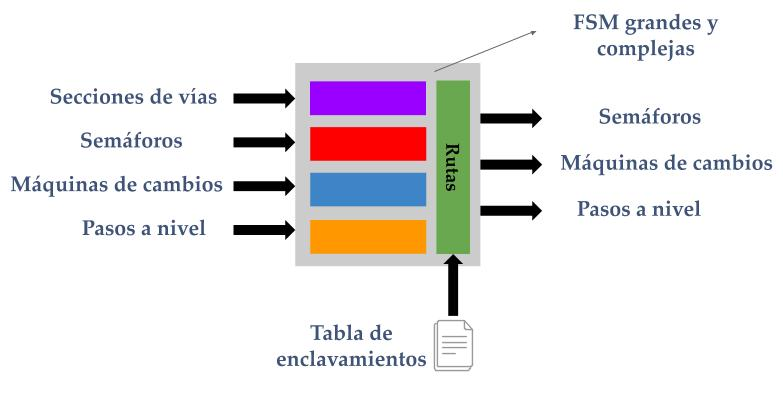
\includegraphics[scale=.65]{./Figures/Funcional}
				\caption{Enfoque funcional.}
				\label{fig:Modelo_Funcional}
			\end{figure}
		
		\vspace{10cm}
		
		Cada bloque horizontal en diferentes colores representa máquinas de estados que modelan los elementos de entrada indicados. Todos ellos, gobernados por una máquina de estados general representada en un bloque se diseña en base a la tabla de enclavamientos (indicado en color verde en la figura \ref{fig:Modelo_Funcional}). 	
		
		La salida del sistema actúa sobre todo el señalamiento, menos la ocupación de los tramos de vías porque son elementos de solo lectura. Puede verse que conforme se añadan mas rutas a la tabla de enclavamientos, las máquinas de estados serán mas complejas y de mayor tamaño.
	
	\subsection{Flujo de trabajo}
		
		En el enfoque funcional, la tabla de enclavamientos es la piedra angular de todo el proceso, sin ella no se puede realizar ningún diseño. En la figura \ref{fig:Work_Funcional} se ilustra el flujo de trabajo para este enfoque.		
			
		\begin{figure}[h]
		\centering
			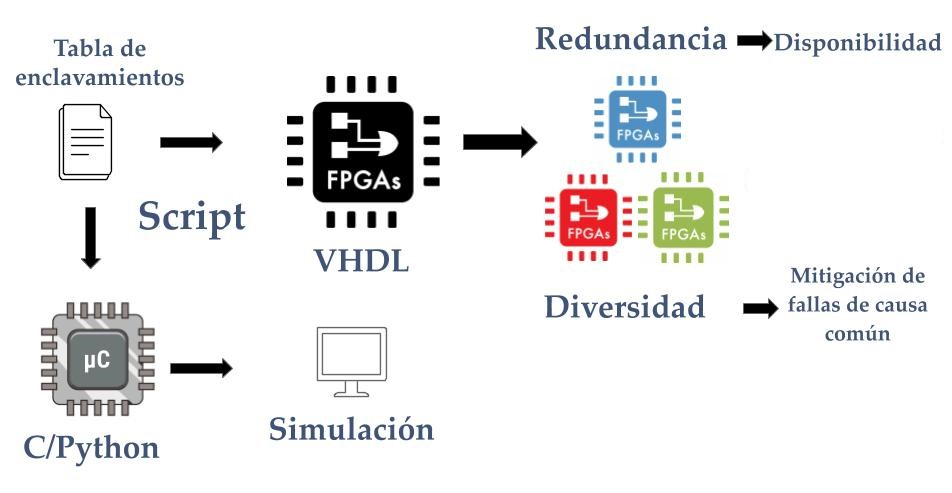
\includegraphics[scale=.5]{./Figures/Funcional_workflow}
			\caption{Esquema de trabajo en el enfoque funcional.}
			\label{fig:Work_Funcional}
		\end{figure}
	
		En la sección \ref{2_2} se resaltó que el diseño nace de la tabla de enclavamientos, y para evitar que cualquier error en esta impacte negativamente en la seguridad del sistema, varios profesionales ferroviarios se encargan de diseñarla y revisarla. Además, su validación puede ser automatizada mediantes \textit{scripts} que busquen errores en las mismas.
		
		El proceso culmina con la redundancia de los sistemas diseñados y la diversificación de plataformas, sin lo cual no se podrían alcanzar los niveles de disponibilidad y seguridad necesarios.
			
		%En el transcurso de la Especialización de Sistemas Embebidos se trabajó en un diseño con enfoque funcional de la estación Belgrano R de la Línea Mitre, pero sin automatización del proceso. En él, la tabla de enclavamientos fue una pieza vital de todo el desarrollo.
				
	\subsection{Escalabilidad de la estrategia}	
		
		Automatizar el proceso de generación del código es inmediato ya que la tabla de enclavamientos define todas las funcionalidades necesarias. Pero al hacerlo se llegó a la conclusión de que los bloques que contenían las máquinas de estados crecen de tamaño hasta volverse inmanejables las conexiones. En la figura \ref{fig:Escala_Funcional} se representa el concepto del crecimiento del sistema conforme la topología se vuelve mas compleja.		
					
		\begin{figure}[h]
		\centering
			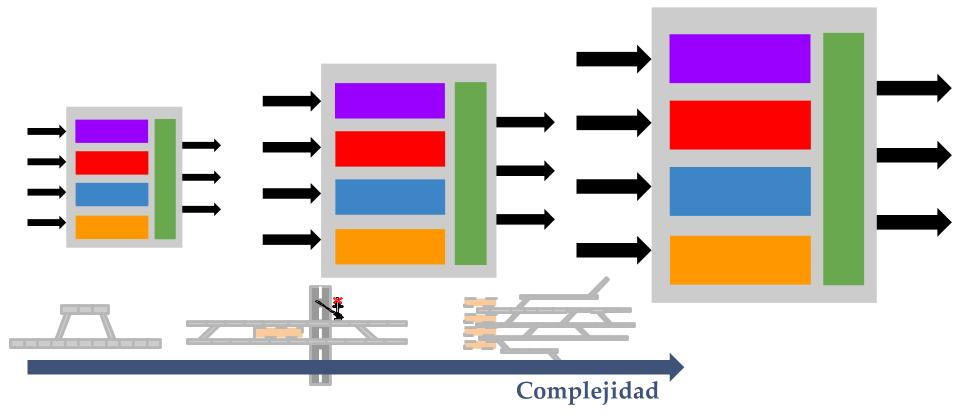
\includegraphics[scale=.5]{./Figures/Funcional_complejidad}
			\caption{Escalabilidad del enfoque funcional.}
			\label{fig:Escala_Funcional}
		\end{figure}
		
	Es importante destacar que a medida que la topología se complejiza la cantidad de bloques para modelarla sigue siendo la misma. Lo que se incrementa es la cantidad de estados en cada bloque y la densidad de conexiones internas y externas a los bloques.
			
	El uso de bloques monolíticos que crecen velozmente perjudica el desarrollo de los tests, los cuales deben ser reescritos por completo cada vez que la topología cambia, incluso ante el cambio más mínimo. 
	
	Otro problema encontrado es el de la incompletitud, que se detalló al inicio de la Sección \ref{Incompletitud}. Si la red admite M rutas pero solo se definieron N como necesarias (donde $N \leq M$), entonces se podrían tener N tests que las validen y el sistema se certifica para N rutas. Pero si en un futuro se necesitan N+1 rutas, se deberá hacer todo el proceso de validación desde cero, lo que encarece todo el proyecto.
			
	La ventaja central de este enfoque es que, teniendo la tabla de enclavamientos correctamente definida, es inmediato pasar de la tabla a la implementación del sistema. La desventaja es que el uso de memoria es excesivo y desde el punto de vista del testing y la validación es incompleto.			
					
\section{Enfoque geográfico}

	En el enfoque geográfico el énfasis está puesto en la interacción entre los componentes a partir de de su posición en la red y no en su funcionalidad a nivel de sistema. Por ende el enfoque geográfico no necesita una tabla de enclavamientos que defina su comportamiento, sino definir genéricamente los componentes y establecer una representación matemática de las conexiones entre ellos. En ese sentido, este enfoque requiere un nivel de análisis previo mucho mayor y, por lo tanto, un mayor tiempo de desarrollo. No obstante, su flexibilidad a la hora de escalar a topologías de mayor tamaño es notable.
	
	Por todo lo expuesto, se remueve el concepto de ruta como elemento central del desarrollo y el foco se pone en modelar los elementos discretos de la red ferroviaria (semáforos, barreras, cambios, circuitos de vía). En la figura \ref{fig:Enfoque_Geografico} se representa la idea central de este enfoque: la variedad de elementos es finita; el foco del desarrollo está centrado en el análisis de la red ferroviaria.
	
		\begin{figure}[h]
		\centering
			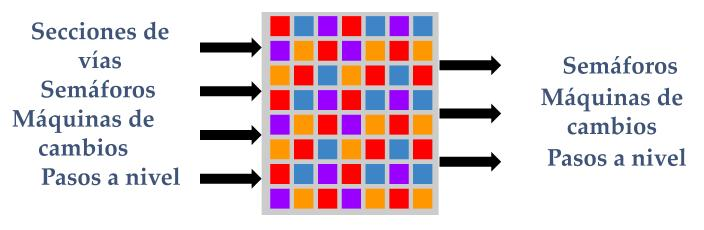
\includegraphics[scale=.55]{./Figures/Geografico}
			\caption{Enfoque geográfico.}
			\label{fig:Enfoque_Geografico}
		\end{figure}

	En la figura \ref{fig:Enfoque_Geografico} los bloques de cada color representan un determinado elemento ferroviario. Así, un bloque cualesquiera se comportará a otro de iguales características y será su posición relativa a los otros bloques lo que determinará la funcionalidad a nivel general.
	
	\subsection{Análisis de grafos}
	\label{grafos}
		Para representar las conexiones entre los elementos ferroviarios, se introduce el concepto de grafo. Un grafo es una representación matemática de las relaciones (aristas) entre componentes (nodos) de una red. Utilizado ampliamente en ciencias de la computación y matemática, es sencillo llegar a un modelo de grafos partiendo desde una topología como la de la figura \ref{fig:Topologia_Grafo}, donde a cada tramo de vía se le asignó un nodo y cada arista del grafo representa el vínculo que existe entre ese tramo y sus vecinos.
		
		\begin{figure}[h]
		\centering
			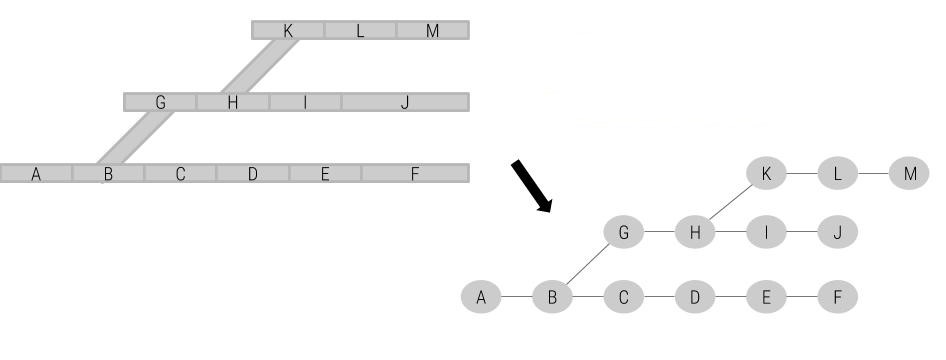
\includegraphics[scale=.4]{./Figures/Topologia_grafo}
			\caption{Pasaje de topología ferroviaria a grafo.}
			\label{fig:Topologia_Grafo}
		\end{figure}
	
		Por ejemplo, el nodo B posee un cambio de vías que vincula los tramos A y C si el cambio se encuentra en posición normal y los tramos A y G si el cambio se encuentra en posición inversa. Por lo tanto, en el grafo, el nodo B posee aristas que lo vinculan con los nodos A,C y G.
		
		La topología de la figura \ref{fig:Topologia_Grafo} puede ser analizada por el algoritmo creado para este trabajo utilizando como información únicamente el grafo que la modela. Todos los nodos que tengan un solo vecino son extremos de la red, mientras que los que tengan tres vecinos se asumirá que poseen un cambio de vías. Los nodos que tengan dos vecinos serán analizados según su posición relativa a cambios cercanos. El resultado de analizar esta topología se muestra en la figura \ref{fig:Grafo_Analisis}.
	
		\begin{figure}[h]
		\centering
			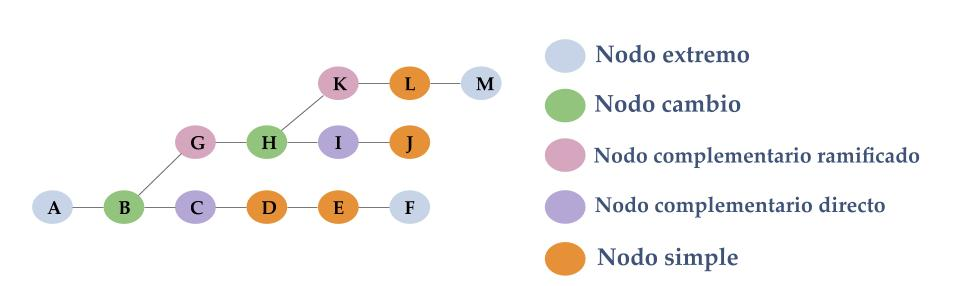
\includegraphics[scale=.4]{./Figures/Grafo}
			\caption{Análisis del grafo ferroviario.}
			\label{fig:Grafo_Analisis}
		\end{figure}
	
		Nodos como el G y el K deben analizarse por su posición relativa a los nodos B y H, que son la raíz del cambio. Al desprenderse de la rama principal de circulación son categorizados como complementos de rama. En cambio los nodos C e I, al continuar el trayecto que tienen los nodos A-B y G-H, son complementos directos de la rama, porque la extienden mas allá de los segmentos indicados.
		
		Otros nodos como D,E y L no tienen ninguna característica especial en este ejemplo, pero bien podrían categorizarse de otra manera si por los tramos de vías que representan se tuviese un paso a nivel.
	
		\subsection{Flujo de trabajo}
		
		El procedimiento se puede repetir para cualquier topología, ya que sin importar la cantidad de elementos o sus conexiones todos los vínculos entre componentes pueden ser representados mediante un grafo. En la figura \ref{fig:Work_Geografico} se ilustra el esquema de trabajo seguido para el enfoque geográfico.	
		
		\begin{figure}[h]
		\centering
			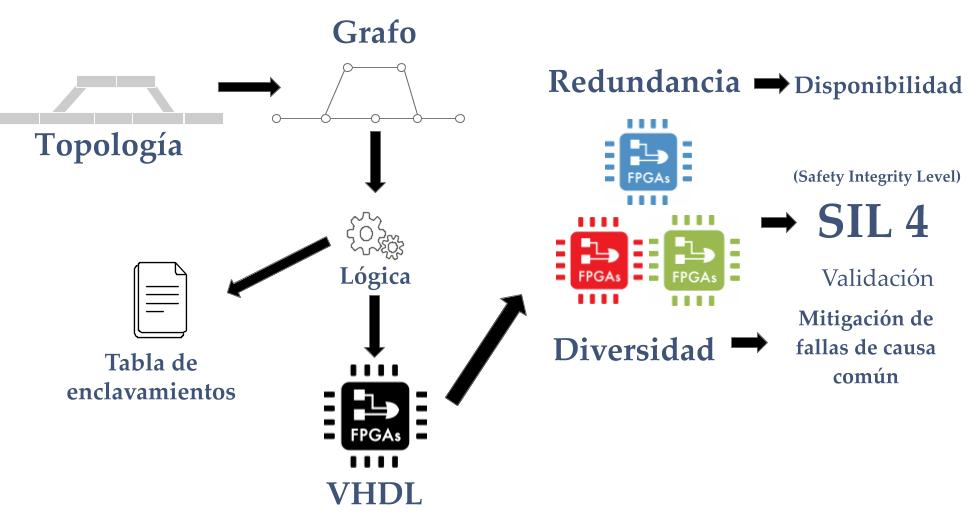
\includegraphics[scale=.5]{./Figures/Geografico_workflow}
			\caption{Esquema de trabajo en el enfoque geográfico.}
			\label{fig:Work_Geografico}
		\end{figure}
	
		A diferencia del enfoque funcional, en el enfoque geográfico la tabla de enclavamientos ocupa un rol secundario al ser un historial del proceso de conversión entre el gráfico y la implementación electrónica del sistema. La tabla de enclavamientos del enfoque funcional (al ser incompleta) debe estar contenida en la tabla de enclavamientos del enfoque geográfico, al considerar todas las rutas que admite la red. Aunque ambos enfoques parten de conceptos distintos, deben converger y brindar resultados comparables, cuya consistencia pueda ser comprobada.
		
		El proceso de implementación de la solución a un sistema ferroviario mediante el enfoque geográfico se inicia con el pasaje del layout al grafo. Este es analizado por el algoritmo que detecta cuántos semáforos, de cuántos aspectos, en qué orientación y dónde deben situarse para que el sistema sea seguro. Esto, además de detectar la posición de todos los cambios y barreras, permite encontrar todas las rutas soportadas por la red y genera como resultado una tabla de enclavamientos completa.
		
		El proceso culmina de forma idéntica al enfoque funcional: aplicando estrategias de redundancia y diversidad se buscará alcanzar un nivel de nivel de disponibilidad y seguridad apropiado.
		
		\subsection{Escalabilidad de la estrategia}	
			
			En el caso del enfoque geográfico el análisis de escalabilidad da un resultado muy diferente al obtenido para el enfoque funcional. En el enfoque geográfico al aumentar la complejidad y tamaño de las topologías, el tamaño de cada bloque se mantiene constante.  Lo que se incrementa es la cantidad de bloques necesarios para implementar el sistema. Esto es ilustrado en la figura \ref{fig:Escala_Geografico}.
					
			\begin{figure}[h]
			\centering
				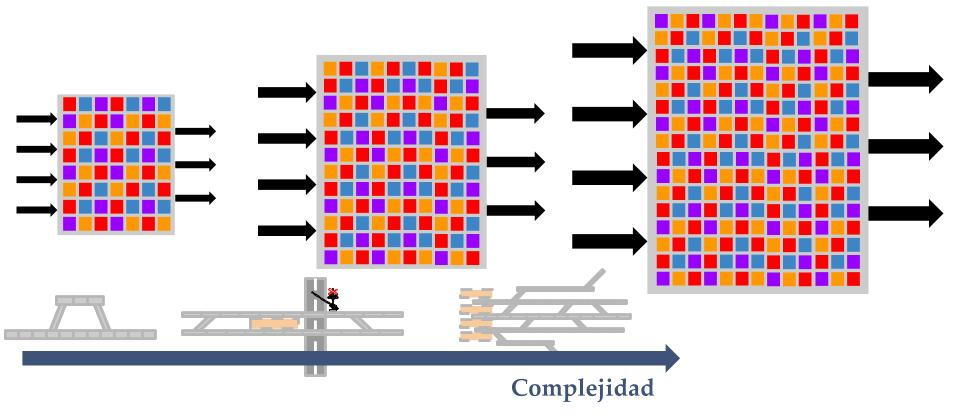
\includegraphics[scale=.5]{./Figures/Geografico_complejidad}
				\caption{Escalabilidad del enfoque geográfico.}
				\label{fig:Escala_Geografico}
			\end{figure}
		
			%\vspace{5cm}
			
			Todos los tests unitarios, referidos a cada bloque del mismo color que modelan un mismo espacio físico (que puede o no contener una barrera, un cambio o varios semáforos). De esta forma se elaboran una única vez, sin importar la cantidad de elementos idénticos presentes en la topología. Sumado a que, como en este enfoque se identifican todas las rutas y por lo tanto se pueden generar todos los tests necesarios, la batería de ensayos que otorga este enfoque es completa. Es decir, siempre se tendrá una cantidad de tests mayor o igual que la necesaria para cualquier necesidad presente o futura.
		
			Una desventaja de este enfoque es que se debe implementar el analizador de redes ferroviarias y un conversor que a partir de un grafo genere toda la estructura de archivos necesaria para implementar el circuito electrónico en una FPGA. Ya que no existen esas herramientas para uso masivo. Por lo tanto, la complejidad y, en consecuencia, el tiempo de desarrollo son mayores.
			
\section{Consideraciones generales}

	En el presente trabajo se optó por implementar el sistema bajo el enfoque geográfico, dado que se consideró que sus ventajas superan a sus desventajas, en particular en lo referente a la mayor escalabilidad y reusabilidad que provee.

	Los módulos del sistema fueron implementados con máquinas de estado finitas con camino de datos (FSMD, del inglés \textit{Finite State Machine with Data path}), que son máquinas de estado finitas (FSM, del inglés \textit{Finite State Machine}) y circuitos secuenciales y combinacionales que constituyen el camino de datos. La FSMD (figura \ref{fig:FSMD}) posee dos partes diferenciadas: el camino de control y el camino de datos. El camino de control se compone de una FSM que, según las entradas de control y el estado interno que posee, genera señales internas que controlan los circuitos secuenciales del camino de datos. Estos, a su vez, contienen los bloques que procesan las entradas y actúan sobre las salidas.

	\begin{figure}[h]
	\centering
		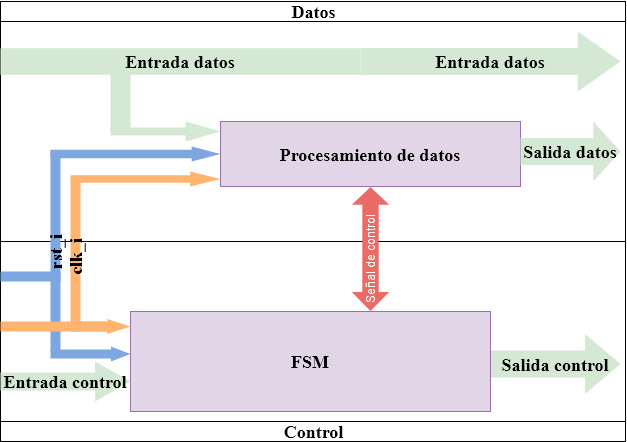
\includegraphics[scale=.55]{./Figures/FSMD}
		\caption{Diagrama en bloques genérico de una FSMD}
		\label{fig:FSMD}
	\end{figure}
	
	%\vspace{5cm}
	
	Siguiendo los lineamientos recomendados, una FSMD debe ser diseñada, implementada y simulada de acuerdo con los siguientes pasos:
	
	\begin{enumerate}
		\item Definición del algoritmo a implementar.
		\item Definición de entradas y salidas de la FSMD.
		\item Diseño del camino de datos.
		\item Diseño de interfaz entre camino de datos y camino de control.
		\item Definición de los estados de la FSM.
		\item Diseño de la FSM.
		\item Implementación del diseño.
		\item Diseño e implementación de los ensayos.
	\end{enumerate}
	
	Esta metodología puede inferir mas tiempo de desarrollo que el habitual, pero ya ha demostrado ser exitosa en el proyecto realizado por el Mg. Ing. Facundo Larosa, codirector de este trabajo. Por lo que se aprovechó su experiencia y conocimiento para resolver esta etapa del desarrollo. Los beneficios son un mayor control del diseño a bajo nivel, una mayor portabilidad y un mas eficiente uso de los recursos de la plataforma electrónica.

	%\vspace{5cm}

\section{Plataforma utilizada}

	Se utilizó una plataforma FPGA, a diferencia de las empresas mencionadas en el capítulo 1 que utilizan microprocesadores, ya que se busca aprovechar la concurrencia y mayor seguridad inherentes a esta tecnología \cite{cite23,cite24,cite25} para la implementación de sistemas
críticos.

	Por razones de disponibilidad se utilizó el kit de desarrollo Arty Z7  (figura \ref{fig:FPGA}), el cual posee 17600 LUT’s, 35200 FF’s, 32 BUFG’s y 100 IOB’s \cite{cite28}. Se lo utilizó como base para sintetizar el diseño y extraer conclusiones que permitan dimensionar los recursos lógicos necesarios para un desarrollo de estas características.
	
	\begin{figure}[h]
	\centering
		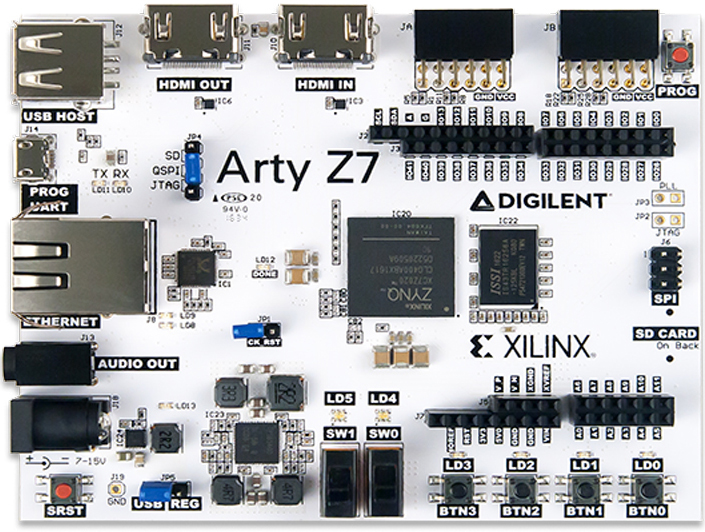
\includegraphics[scale=.55]{./Figures/FPGA}
		\caption{FPGA Arty Z7-10 de Digilent}
	\label{fig:FPGA}	
	\end{figure}			
			
